\documentclass{standalone}
\usepackage{pgfplotstable}
\usepackage{amsmath}
\pagestyle{empty}
\pgfplotsset{compat=1.9}

%this ueses the data files figWaveOctaveWaterDielectricLossEW.txt 
%and figWaveOctaveWaterDielectricLossLFW.txt prepared by octave's
%figWaveOctaveWaterDielectricLoss.m

\begin{document}
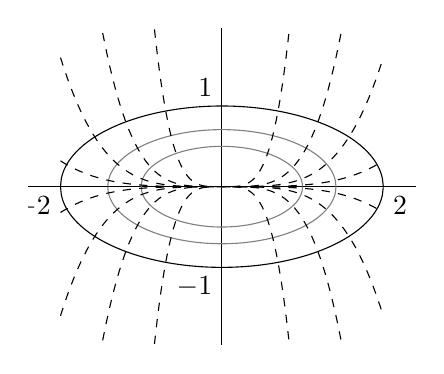
\begin{tikzpicture}[]
\begin{axis}[small,axis equal,axis lines*=middle,scaled x ticks=false,scaled y ticks=false,ymax=1,ymin=-1,xtick=\empty,ytick=\empty]

\pgfmathsetmacro{\ca}{1}
\pgfmathsetmacro{\lmta}{sqrt(4*\ca)}
\addplot[domain=-\lmta:\lmta,samples=400]{sqrt(\ca-x^2/4)};
\addplot[domain=-\lmta:\lmta,samples=400]{-sqrt(\ca-x^2/4)};

\pgfmathsetmacro{\ca}{0.5}
\pgfmathsetmacro{\lmta}{sqrt(4*\ca)}
\addplot[gray,domain=-\lmta:\lmta,samples=400]{sqrt(\ca-x^2/4)};
\addplot[gray,domain=-\lmta:\lmta,samples=400]{-sqrt(\ca-x^2/4)};

\pgfmathsetmacro{\ca}{0.25}
\pgfmathsetmacro{\lmta}{sqrt(4*\ca)}
\addplot[gray,domain=-\lmta:\lmta,samples=400]{sqrt(\ca-x^2/4)};
\addplot[gray,domain=-\lmta:\lmta,samples=400]{-sqrt(\ca-x^2/4)};

\addplot[dashed,domain=-2:2,samples=100]{0.02*x^4};
\addplot[dashed,domain=-2:2,samples=100]{0.1*x^4};
\addplot[dashed,domain=-2:2,samples=100]{0.4*x^4};
\addplot[dashed,domain=-1:1,samples=100]{4*x^4};

\addplot[dashed,domain=-2:2,samples=100]{-0.02*x^4};
\addplot[dashed,domain=-2:2,samples=100]{-0.1*x^4};
\addplot[dashed,domain=-2:2,samples=100]{-0.4*x^4};
\addplot[dashed,domain=-1:1,samples=100]{-4*x^4};

\addplot[] plot coordinates {(2,0)}node[below right]{$2$};
\addplot[] plot coordinates {(-2,0)}node[below left]{$-2$};
\addplot[] plot coordinates {(0,1)}node[above left]{$1$};
\addplot[] plot coordinates {(0,-1)}node[below left]{$-1$};
\end{axis}%
%
\end{tikzpicture}%

\end{document}
